\documentclass[dvipdfmx]{jarticle}
\usepackage{fancyvrb}
\setlength{\textheight}{23.5cm}
\usepackage{tikz}
\usetikzlibrary{automata,calc,shapes}
\usepackage{tabularx}
\pagestyle{empty}
\newcounter{coffee}
\newcounter{bean}
\begin{document}
\begin{center}
  {\bf\Large コンパイラ演習課題(3)(解答例)}
\end{center}
\begin{list}{[\arabic{coffee}]}{\usecounter{coffee}}
    \item 生成規則に以下のような番号をつけ，$\mathsf{First}_1$, $\mathsf{Follow}_1$は以下のようになる．

    \begin{tabularx}{.8\textwidth}{m{.2\textwidth}m{.3\textwidth}m{.3\textwidth}}
    
\includegraphics{answer-colab/g1-rules.pdf}
    & 
    
\includegraphics{answer-colab/g1-first.pdf}
    &
    
\includegraphics{answer-colab/g1-follow.pdf}
    \end{tabularx}

    LL(1)の下向き構文解析表およびLALR(1)構文解析表は以下のように構成される．

    \begin{tabularx}{\textwidth}{m{.4\textwidth}m{.6\textwidth}}
    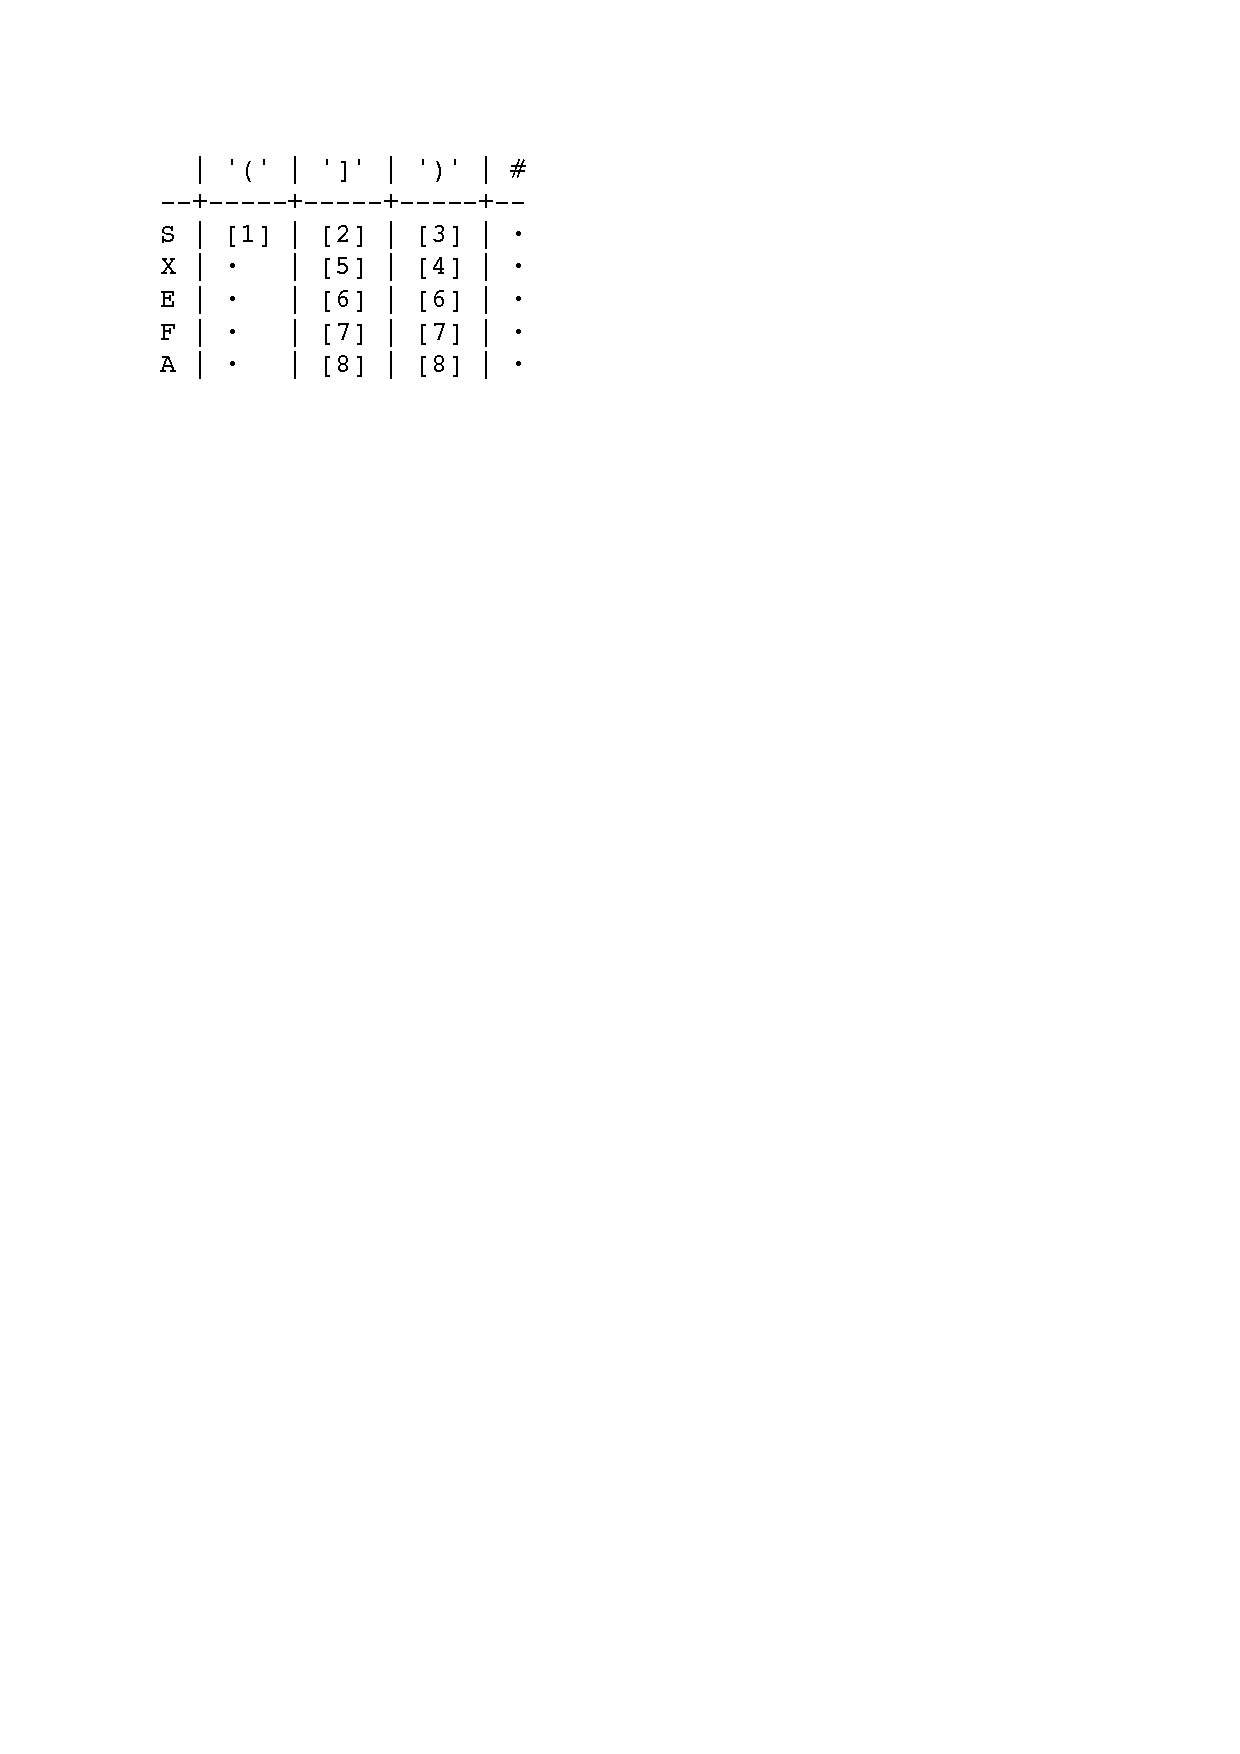
\includegraphics[width=.4\textwidth]{answer-colab/g1-LL1table.pdf}
    &
    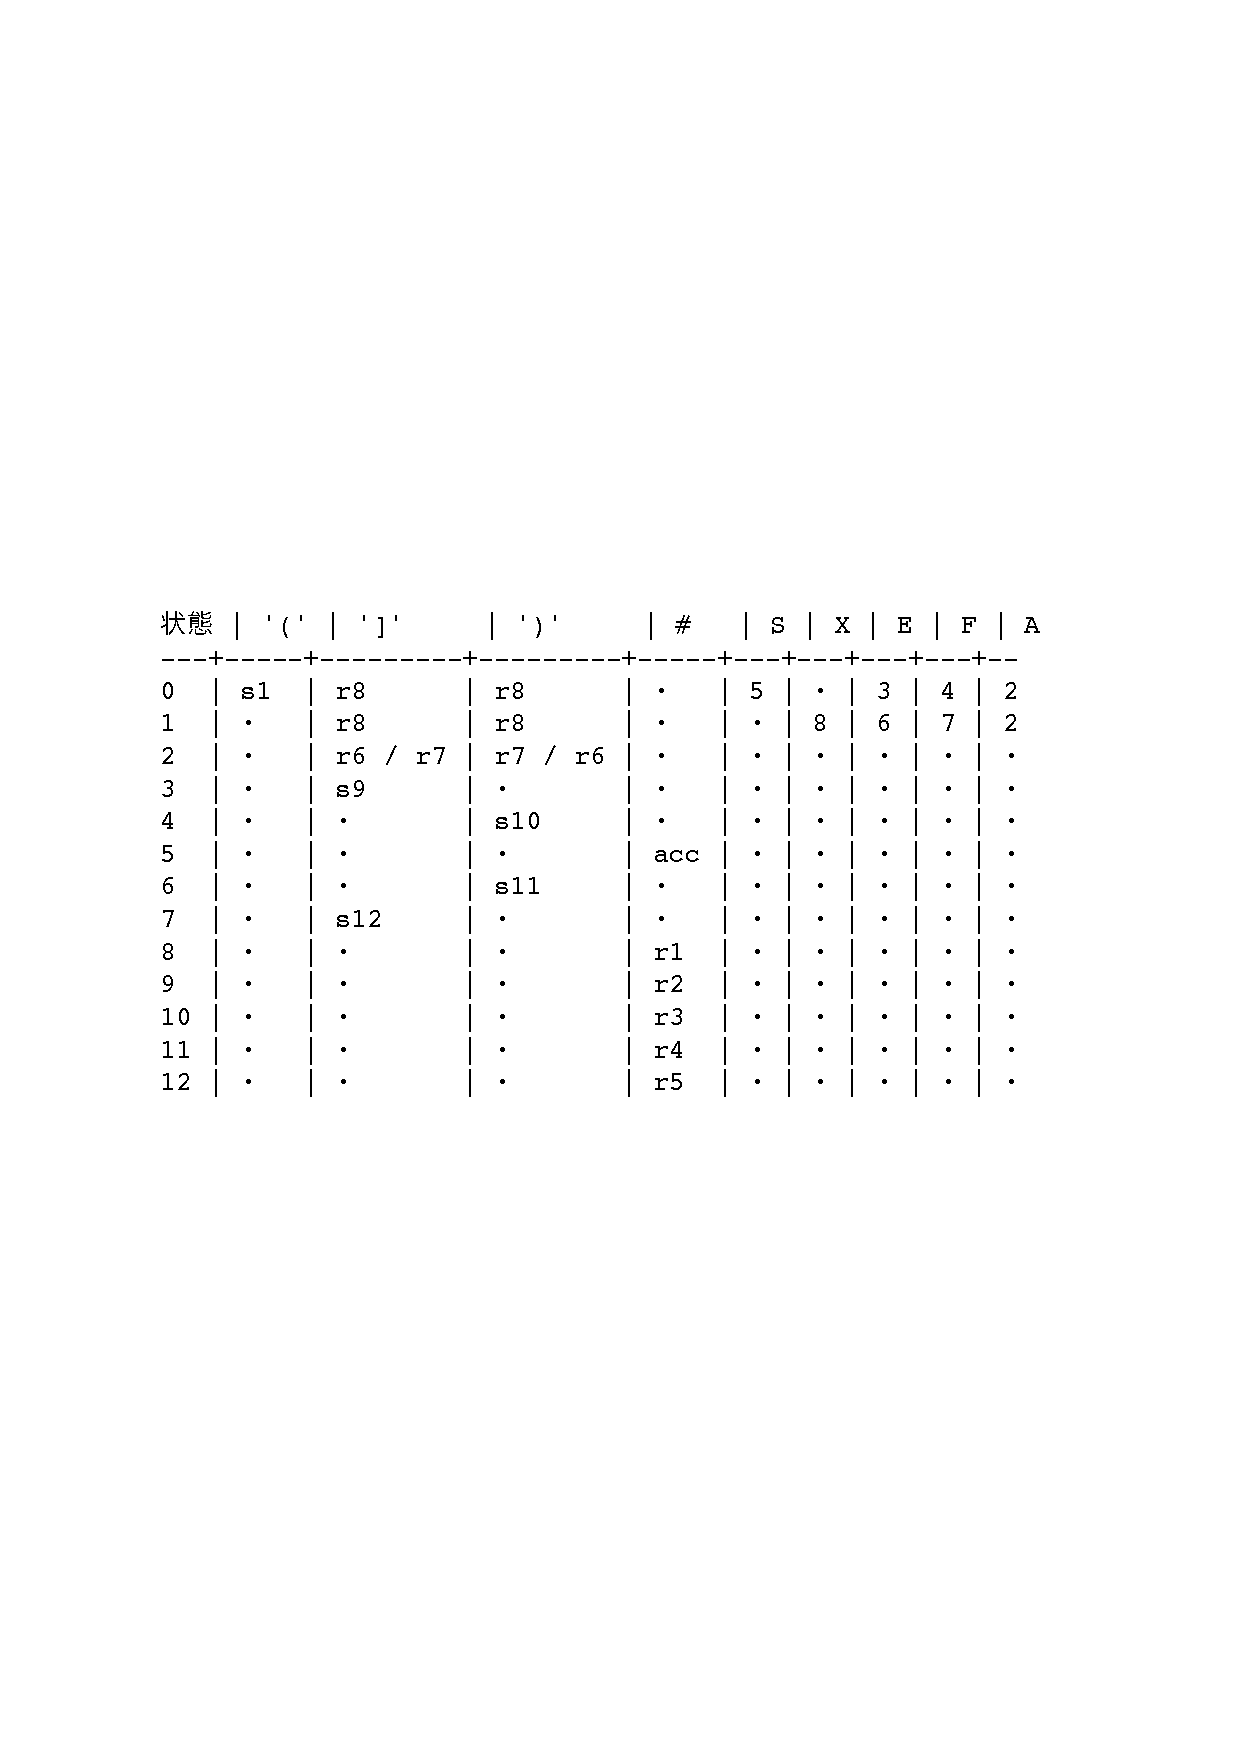
\includegraphics[scale=0.4]{answer-colab/g1-LALR1-table.pdf}
    \end{tabularx}

    r6/r7 で$A$を$E$に還元すればよいか$F$に還元すればよいかを判断できないので，LALR(1)ではない．
    これに対して下向き構文解析は，$A$のFollowで規則を判断できる．
    \item 
    \begin{list}{(\alph{bean})}{\usecounter{bean}}
        \item LALR(1)構文解析表は以下のようになる．
        \begin{center}
        \begin{tabularx}{.9\textwidth}{m{.3\textwidth}m{.6\textwidth}}
            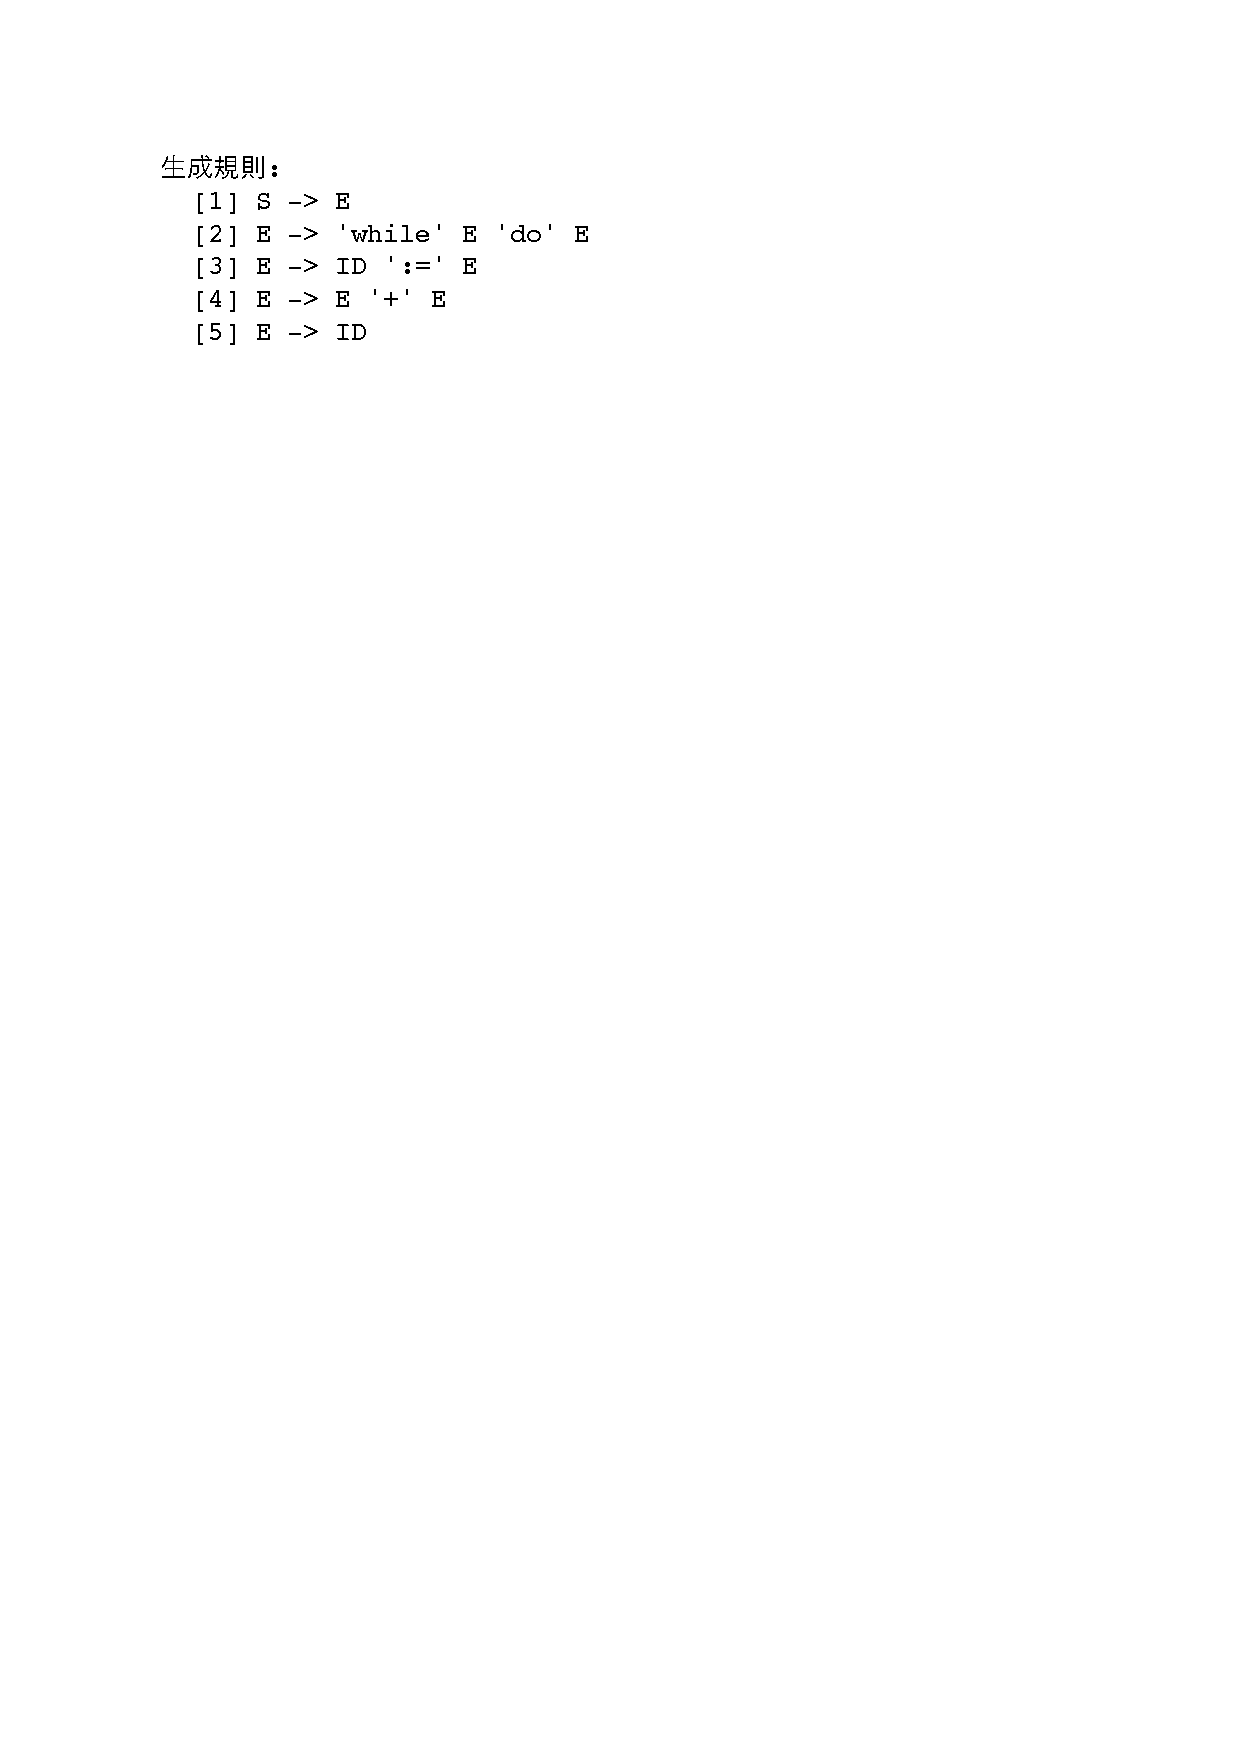
\includegraphics[width=.3\textwidth]{answer-colab/g2-rules.pdf}
            &
            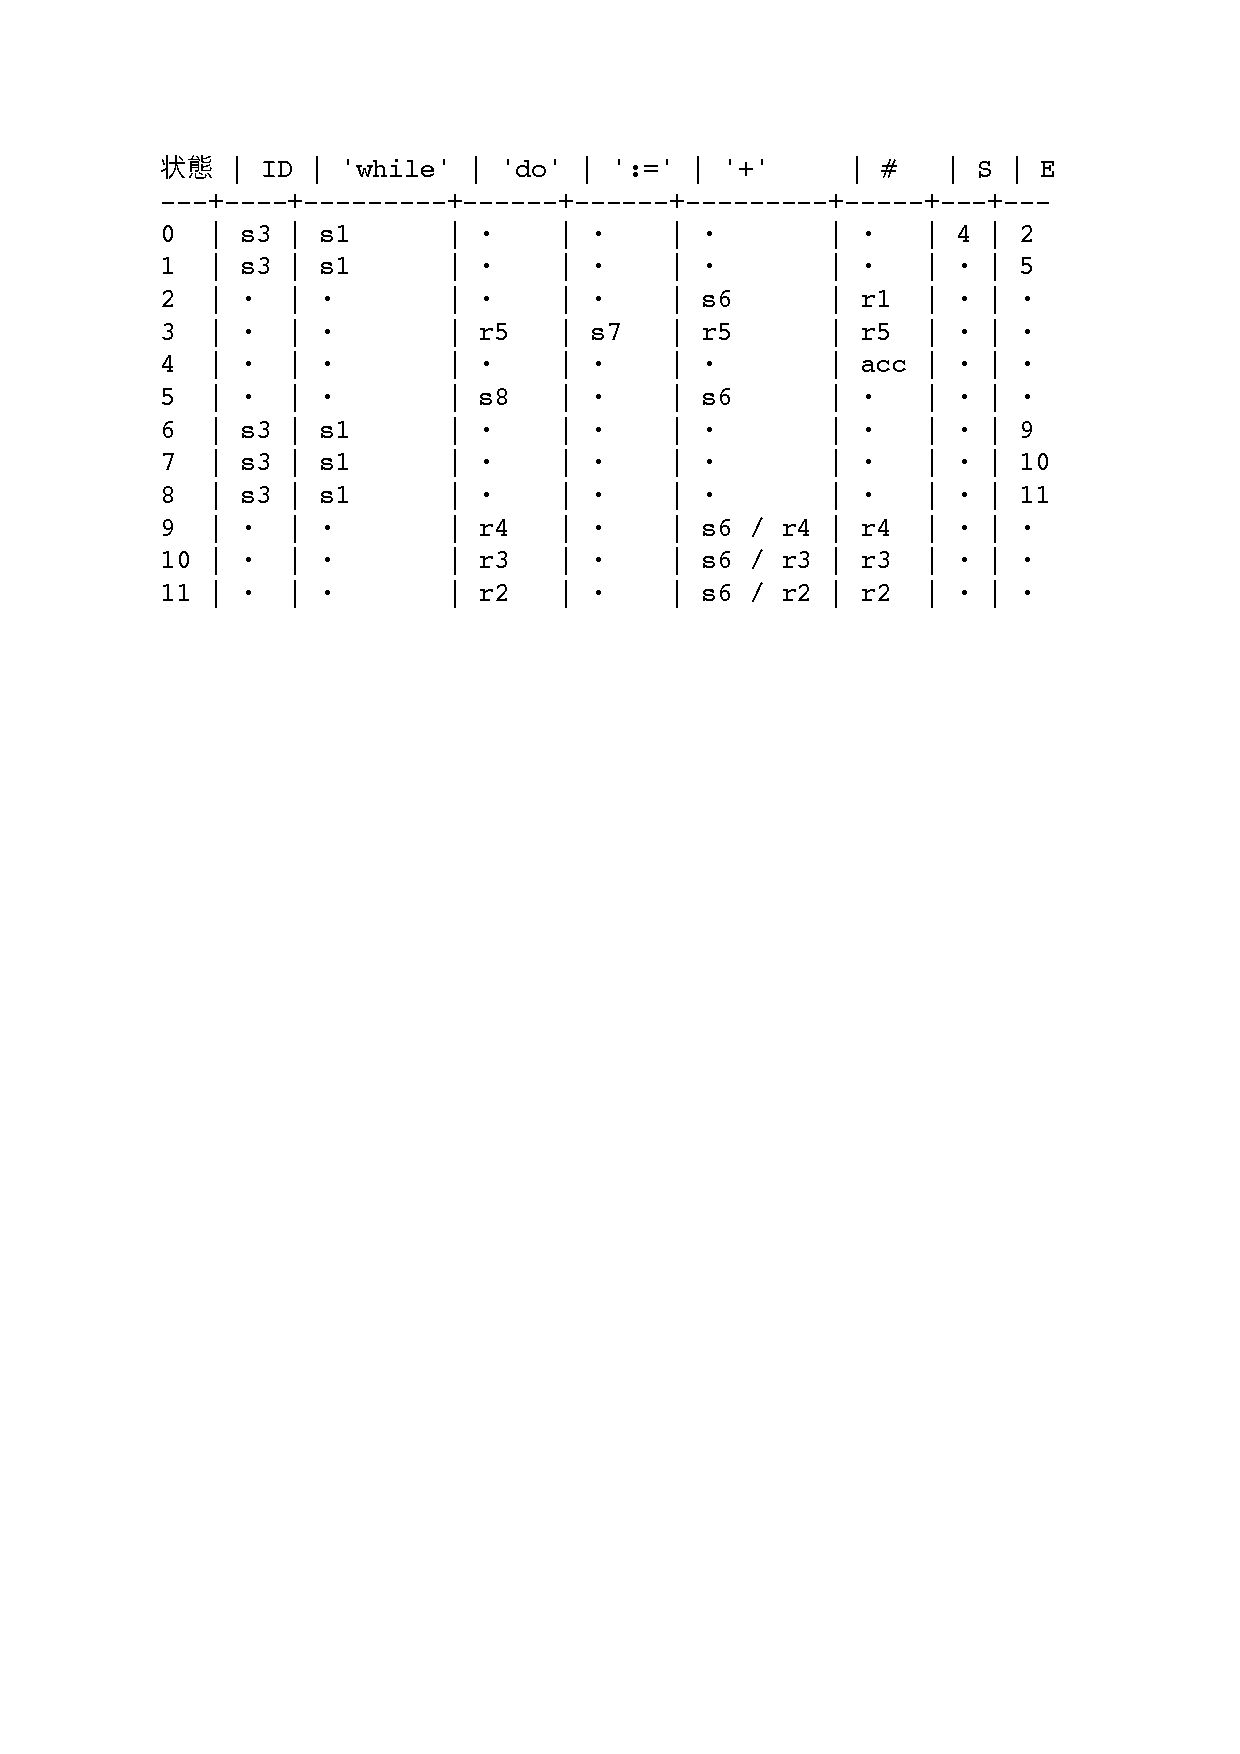
\includegraphics[width=.6\textwidth]{answer-colab/g2-LALR1-table.pdf}
        \end{tabularx}
    \end{center}
    \item 構文解析表で衝突が発生しているのは，$\texttt{+}$が$\texttt{do}$ の範囲内にあるか，範囲外にあるかということがこの文法からは判断できないためである．例えば，\verb|while ID do ID=|$E$\verb| + |$E$の解釈を
    (\verb|while ID do ID=|$E$)\verb| + |$E$とするか，\verb|while ID do |(\verb|ID=|$E$\verb| + |$E$)とするか，の違いである．後者の方が解釈としては自然であるので，衝突が起こっているエントリーでは，シフトを優先して\verb|do|の範囲を大きくする方が自然である．
    \end{list}
    \item 講義ページのチェックツールにおいて，文法を記述すると以下のようになる．
    
    \begin{minipage}{.3\textwidth}
    \begin{Verbatim}[frame=single]
%start S
%%
S : X
  ;
X : M 'a'
  | 'b' M 'c'
  | 'd' 'c'
  | 'b' 'd' 'a'
  ;
M : 'd'
  ;
%%
    \end{Verbatim}
\end{minipage}

上記のファイルを\verb|ex261016g3.y|とする．

\verb|!python3 slr1.py ex261016g3.y|を実行する．

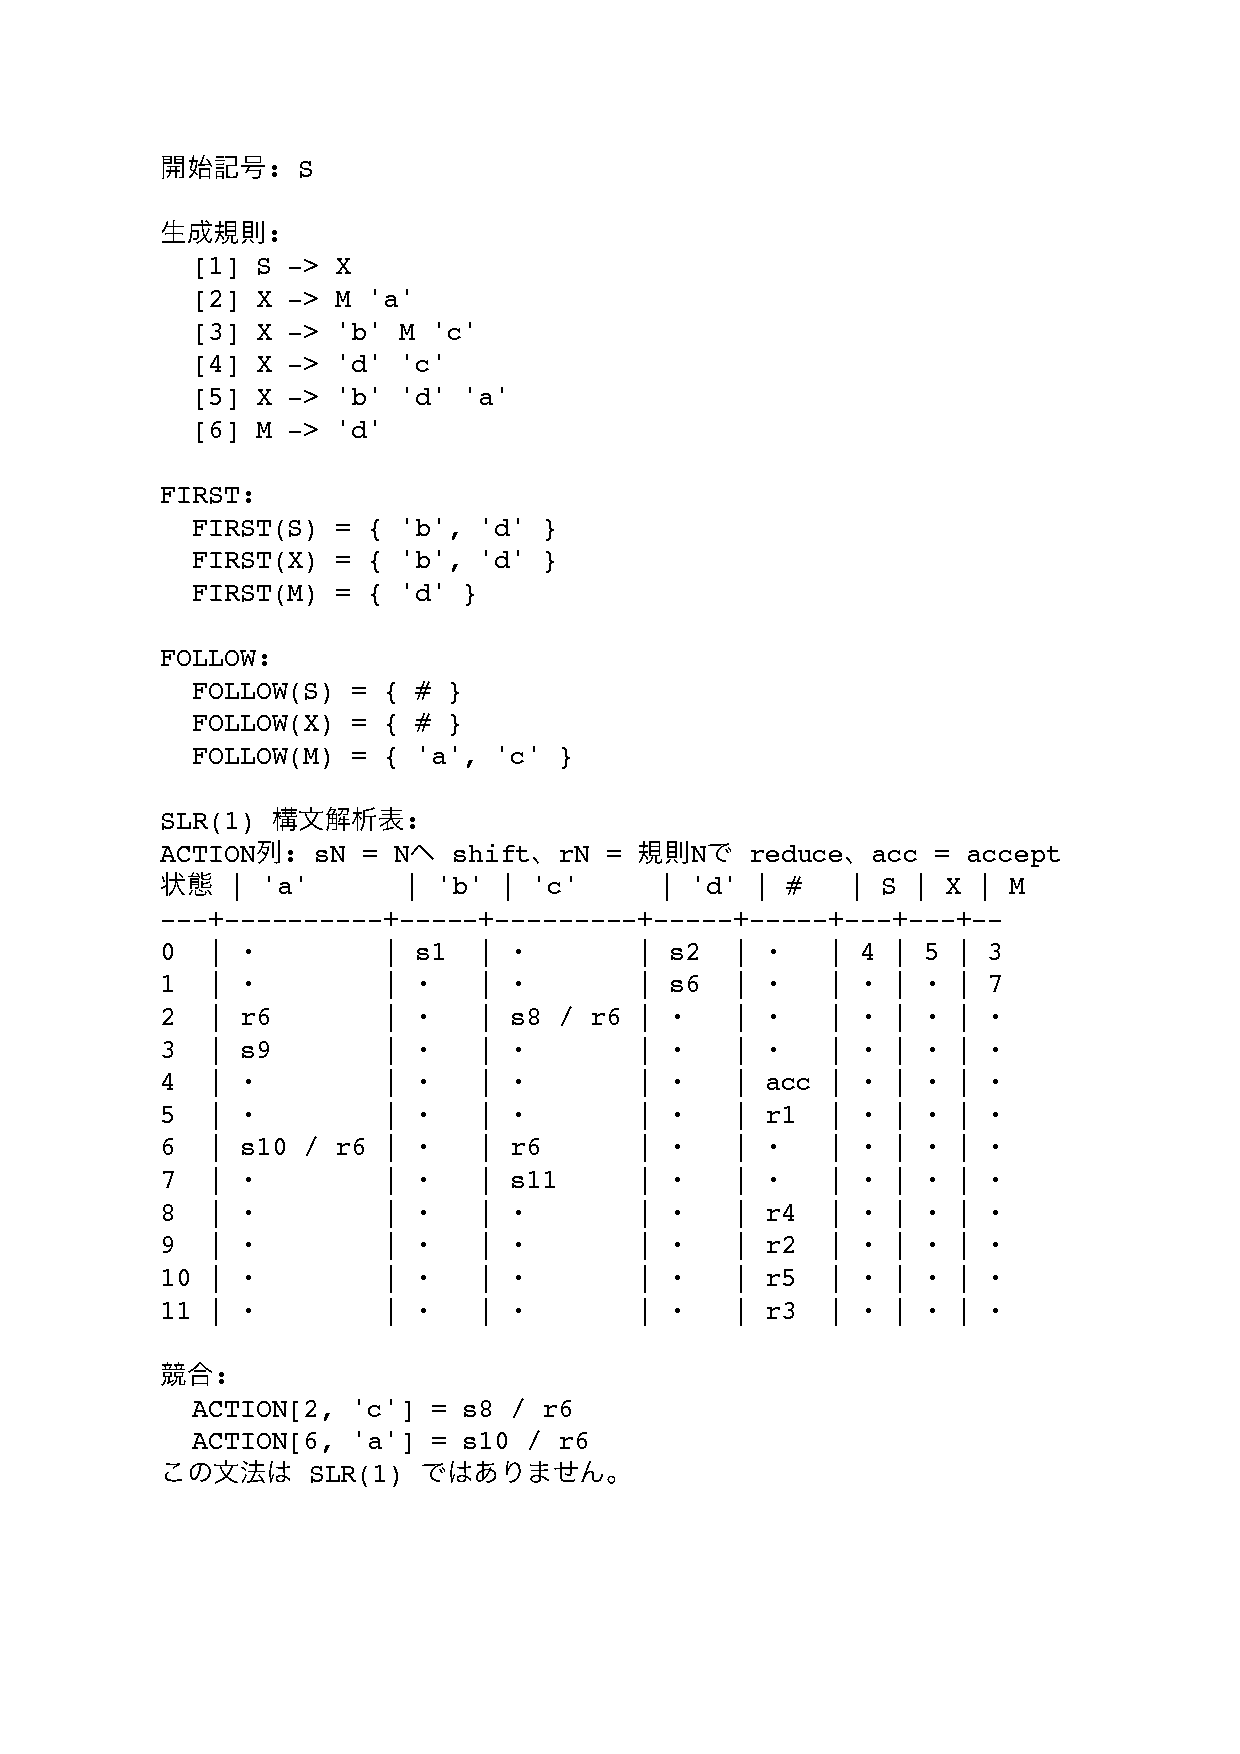
\includegraphics[width=.8\textwidth]{answer-colab/g3-slr1.pdf}

\verb|!python lr11.py ex261016g3.y|を実行すると以下のようになる．

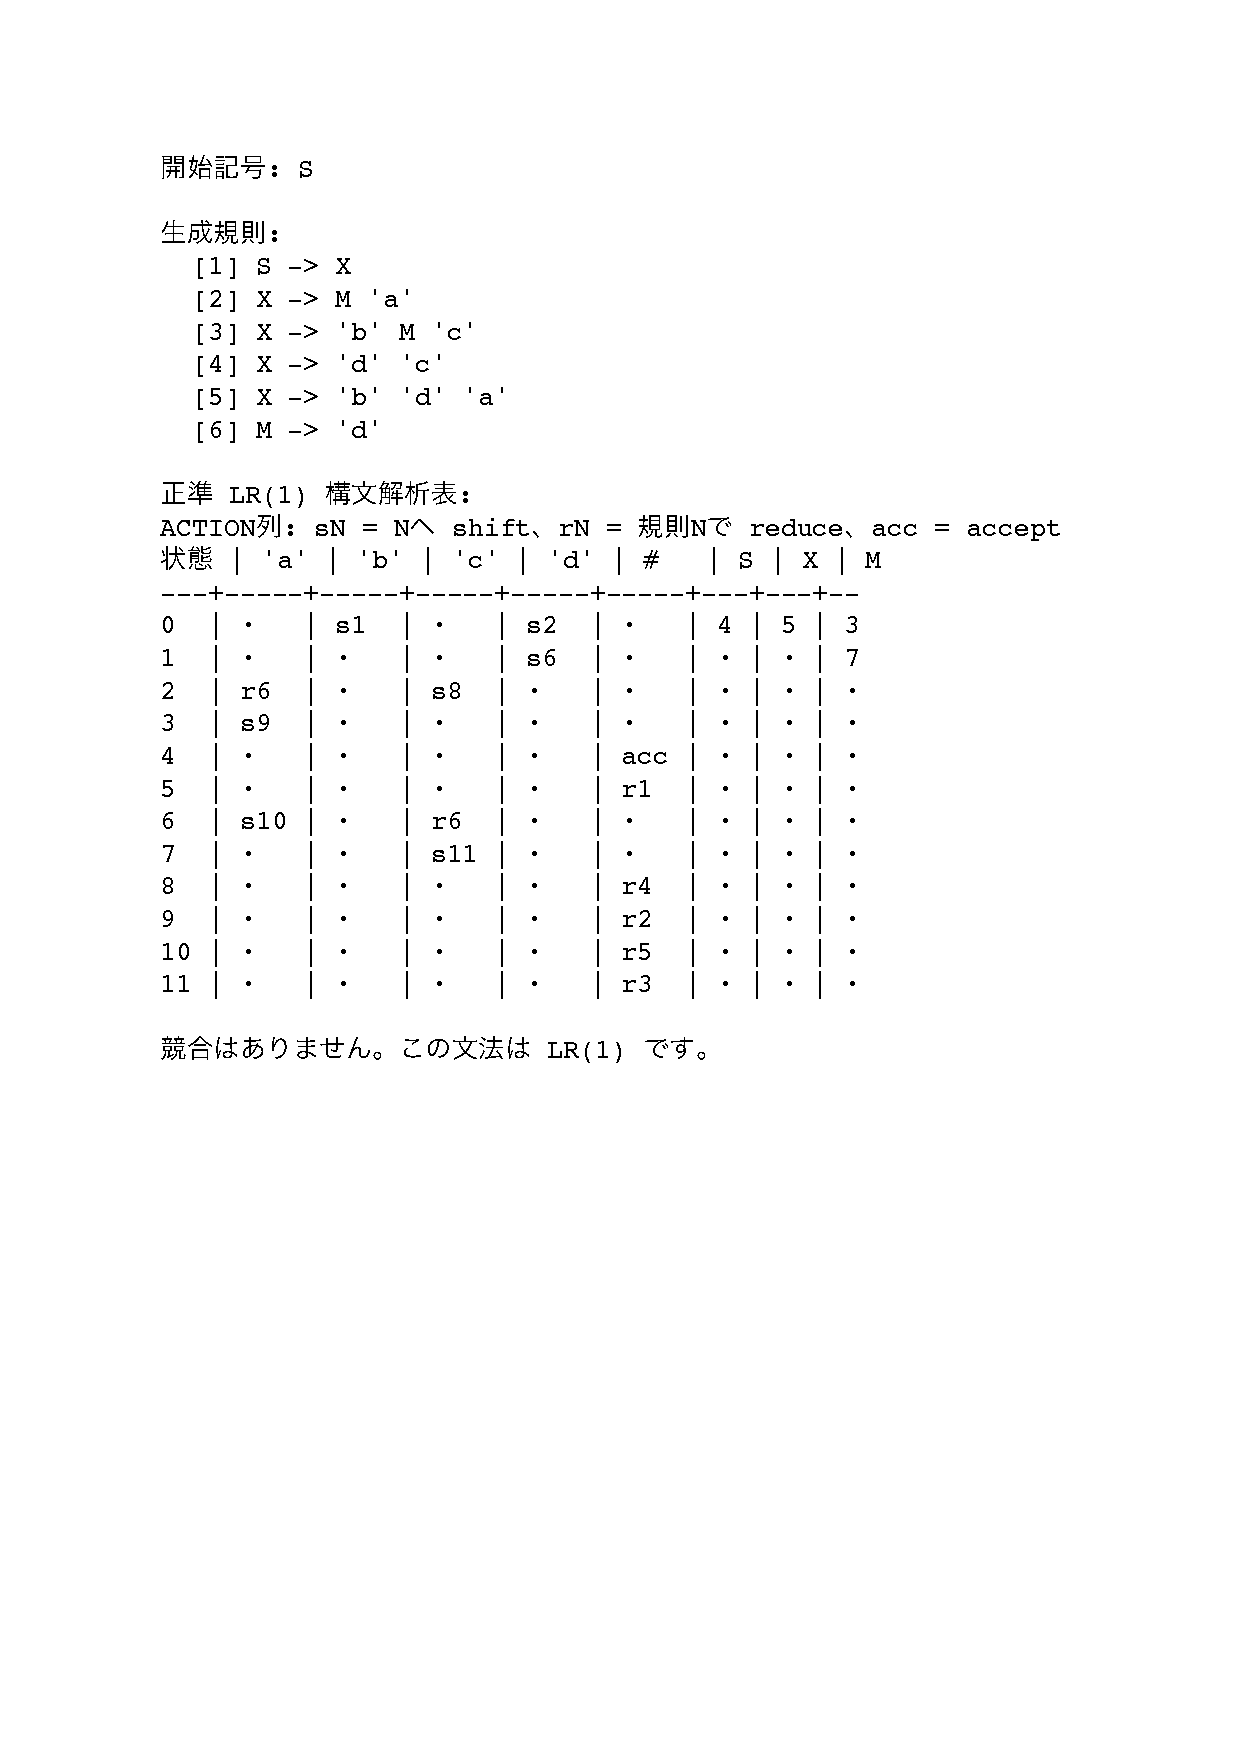
\includegraphics[width=.8\textwidth]{answer-colab/g3-lr1.pdf}

\end{list}
\end{document}